%\documentclass[preprint,12pt]{elsarticle}  % final
\documentclass[paper = letter, fontsize = 11pt]{scrartcl} % double spacing

\usepackage{graphicx}
\usepackage{amssymb}
\usepackage{amsthm}
\usepackage{lineno}
\usepackage{fullpage}
\usepackage{subfig}
\usepackage{soul}
\usepackage{color}
% for inline annotation
\usepackage[colorinlistoftodos]{todonotes}
\usepackage{mathtools}
\usepackage{booktabs}
\usepackage{array}
\usepackage{url}
\usepackage{todonotes}
\usepackage[section]{placeins}
% \usepackage[]{mcode}
\usepackage{listings}
\usepackage[colorlinks=true]{hyperref}


\hypersetup{
    linkcolor=blue
  }
\graphicspath{{./figs/}}


\lstnewenvironment{CPP}
{\lstset{language=C++,
                basicstyle=\ttfamily,
                backgroundcolor=\color{lightgreen},
                breaklines=true, 
                frame=single,
                numbers=left, numberstyle=\footnotesize, stepnumber=1, numbersep=5pt,
                keywordstyle=\color{blue}\ttfamily,
                stringstyle=\color{red}\ttfamily,
                commentstyle=\color{green}\ttfamily,
                morecomment=[l][\color{magenta}]{\#} } }
  {}

\lstnewenvironment{python}
{\lstset{language=Python,
                basicstyle=\ttfamily,
                backgroundcolor=\color{lightcyan},
                breaklines=true, 
                frame=single,
                numbers=left, numberstyle=\footnotesize, stepnumber=1, numbersep=5pt,
                keywordstyle=\color{blue}\ttfamily,
                stringstyle=\color{red}\ttfamily,
                commentstyle=\color{red}\ttfamily,
                morecomment=[l][\color{magenta}]{\#} }
}
{}


% define colors
%% see: http://latexcolor.com/
\definecolor{lightgreen}{rgb}{0.56, 0.93, 0.56}
\definecolor{lightpink}{rgb}{1.0, 0.71, 0.76}
\definecolor{lightblue}{rgb}{.90,.95,1}
\definecolor{darkgreen}{rgb}{0,.5,0.5}
\definecolor{lightcyan}{rgb}{0.88, 1.0, 1.0}


%indicates who is to lead the work
%input #1: summary of entry
%input #2 is a list of names
%input #3 is the description and guide of the task

\newcommand\assignment[3]{\todo[inline,color=red!30,size=\small,caption={#1}]{\textbf{#2's task}: #3}}

%indicates the status of the work
%input #1: summary of entry, be short
%input #2 is a list of names
%input #3 is the description and status of the completed work

\newcommand\statusreport[3]{\todo[inline,color=blue!30,size=\small,caption={#1}]{\textbf{Status from #2}: #3}}

% comments
%input #1: summary of entry, be short
%input #2 is name of the commentator 
%input #3 is the comments

\newcommand\commof[3]{\todo[inline,backgroundcolor=green!50,size=\small,caption={#1}]{{\color{blue} {#2}'s comments}: #3}}



\newcommand\norm[1]{\left\lVert#1\right\rVert}
\newcolumntype{C}[1]{>{\centering\arraybackslash}p{#1}}

%% natbib.sty is loaded by default.


\begin{document}
\makeatletter

\setlength{\@fptop}{0pt}
\makeatother

\title{Model Form Uncertainty Quantification in RANS: Technical Details}
\author{Jinlong Wu, Jianxun Wang, Rui Sun, and Heng Xiao} 

\maketitle
\tableofcontents
\listoftodos

\section*{Overall Guidelines and Rules of Collaboration}
\begin{itemize}
\item Identify your items and complete your task.
\item Report your progress under the \verb+\statusreport+ environment, and include essential results
  in this document.
\item Talk to other team members often to ensure smooth interfacing.
\item Take ``unit testing'' seriously. Other members rely on the correctness of your code to
  proceed. This is standard software engineering practice.  All modules in MUQ (both in C++ and
  Python) come with unit tests\footnote{MUQ-v0.1/MUQ/modules/}. See
  \url{MUQ-v0.1/MUQ/modules/Geostatistics/test} for example. \textbf{Follow these examples for write
  your unit testing code.}
\item Configure on “repositoryhosting” dashboard so that you receive email whenever there is a
  ``commit to the repository''.
\end{itemize}

Specific rules of using git for \LaTeX version control:
\begin{itemize}
 \item Always pull before making any changes.
 \item Commit and push to repository frequently.
 \item Document any significant work frequencly in latex. Remember to commit figures and bibliography
   files as well.  Latex or Beamer are both acceptable for such documentations.  
 \item Resolve any changes locally first before
   committing to repository.  
   \item Configure your editor to wrap latex documents to 100 characters per line!
\end{itemize}

Finally, this is an experiment of group collaboration. The success of this effort depends on
contributions from all members. The present order of authors are preliminary.  Final authorship
should fairly reflect each member's respective contribution. 

The current plan is to finish the majority of the tasks by the end of the semester, and submit as
final project of the class ``Turbulence Modeling and Simulation''. I will write a report to Dr. Roy
about each member's contributions.



\section{Modification of RANS Solver}

\assignment{JL/Rui: Modify RANS solver for given $\tau_{ij}$}{JL/Rui}{Implement and test the RANS solver wit specified
  Reynolds stress field.}

 \statusreport{JL/Rui: In progress}{JL/Rui}{}

The momentum equation read as follows:

\begin{CPP}
    tmp<fvVectorMatrix> UEqn
    (
        fvm::div(phi, U)
      + turbulence->divDevReff(U)
      ==
        fvOptions(U)
    );
\end{CPP}

The key term here is \verb+turbulence->divDevReff+, which gives the divergence of the Reynolds
stress $\langle u'_i u'_j \rangle$.  Two examples of the implementation of this function are as
follows. The first is from an eddy-viscosity model ($k$--$\varepsilon$); the second is from a
Reynolds stress transport model (LRR).  In the $k$--$\varepsilon$ code, line 6, that is,
\verb+- fvc::div(nuEff()*dev(T(fvc::grad(U))))+ corresponds to numerical error.  In the LRR code, it
is easier to look at lines 21--23.  The terms in line 22 and 23,
\verb&fvc::laplacian(nut_, U, "laplacian(nuEff, U)") - fvm::laplacian(nuEff(), U)& is to recover
laminar stresses. However, the term with \verb+-fvm::laplacian(nuEff(), U)+ is to enhance stability
by adding a diffusion term that is treated explicitly. Consider the central differencing stencil of
the diffusion term, and the fact that the term \verb+divDevReff+ has a positive sign in the momentum
equation.

The intention of \verb+couplingFactor+ (which must be between 0 and 1; default is 0) is not clear
right now.  We will take it as 0.

\begin{CPP}
  tmp<fvVectorMatrix> kEpsilon::divDevReff(volVectorField& U) const { return ( -
    fvm::laplacian(nuEff(), U) - fvc::div(nuEff()*dev(T(fvc::grad(U)))) ); }
\end{CPP}

\begin{CPP}
tmp<fvVectorMatrix> LRR::divDevReff(volVectorField& U) const
{
    if (couplingFactor_.value() > 0.0)
    {
        return
        (
            fvc::div(R_ + couplingFactor_*nut_*fvc::grad(U), "div(R)")
          + fvc::laplacian
            (
                 (1.0 - couplingFactor_)*nut_,
                 U,
                 "laplacian(nuEff,U)"
            )
          - fvm::laplacian(nuEff(), U)
        );
    }
    else
    {
        return
        (
            fvc::div(R_)
          + fvc::laplacian(nut_, U, "laplacian(nuEff,U)")
          - fvm::laplacian(nuEff(), U)
        );
    }
}
\end{CPP}


\section{Physics-Based Parameterization and Perturbation of Reynolds Stresses}

\subsection{Theory}
\commof{XH: Document nontrivial theories.}{XH}{In this section, document the non-trivial theories
  behind the implementations, e.g., the Baycentric mapping. Refer to literature if applicable.}

\subsection{Implementation Plan}
This part deals with the perturbation of the Reynolds stress obtained from the RANS
simulations. Specifically, we need to implement and test the following functions:

\assignment{JL/Rui: Reynolds stress mapping}{JL/Rui}{Implement and test the following functions in Items 1--3.}
\statusreport{JL/Rui: In progress}{JL/Rui}{}

\begin{enumerate}
\item Mapping from Reynolds stress $\tau_{ij}$ to physical parameters $k, C_2, C_3, v_1, v_2, v_3$
\begin{python}
def tau2PhysParams(taus):
    """
    Input: 
    taus: a list/array of Reynolds stresses
    Return:
    a list/array of the structure (k, C2, C3, v1, v2, v3)
    """
      \end{python}
\item Mapping from  physical parameters $k, C_2, C_3, v_1, v_2, v_3$ to Reynolds stress $\tau_{ij}$
\begin{python}
def physParams2Tau(params):
    """
    Input:
    List/array of parameters (k, C2, C3, v1, v2, v3)
    Return: 
    List/array of  Reynolds stresses (taus)
    """
  \end{python}

\item Perturbation of a given Reynolds stress field by a specified amount in the Baycentric mapping
\begin{python}
def perturbTaus(taus, perturbParams):
    """
    Input:
    -  List/array of Reynolds stresses (taus)
    -  List/array of perturbation parameters (psi, Delta)
    Return:
    perturbed Reynolds stresses (perturbedTau)
    """
\end{python}
\end{enumerate}

Mapping between the equilateral triangle to the unit square is shown in Fig.~\ref{fig:phy-map}.  The set of degenerated 
shape functions are\footnote{Li, L. et al. (2004). Study on the degeneration of quadrilateral element to triangular element. Communications in Numerical Methods in Engineering, 20(9), 671-67. (see Sente)}

\begin{align}
  \label{eq:shapefun}
  N_1(\xi, \eta) & = \frac{(1 + \eta)}{2} \\
  N_3(\xi, \eta) & = \frac{(1 - \xi) (1 - \eta)}{2} \\
  N_4(\xi, \eta) & = \frac{(1 + \xi) (1 + \eta)}{2}
\end{align}
Note the shape function $N_2$ is missing due to the regeneration.  The mapping from computational
coordinate ($\xi, \eta$) to physical coordinate ($x, y$) for an arbitrary point is as follows:
\begin{align}
  x & = x(\xi, \eta) = \sum_{i=1, 3, 4} N_i (\xi, \eta) x_i \\
  y & = y(\xi, \eta) = \sum_{i=1, 3, 4} N_i (\xi, \eta) y_i
\end{align}
where $(x_1, y_1)$, $(x_3, y_3)$, $(x_4, y_4)$ are the physical coordinates of vertex of the
equilateral triangle with $(x_{rans}, y_{rans})$ as the origin. As shown in Fig.~\ref{fig:phy-map},
points 1, 3, and 4 corresponds to 3C (isotropic turbulence), 2CI (2C isotropic turbulence), and 1C,
respectively. The mapping from ($x, y$) to ($\xi, \eta$), if needed, can be obtained by inverting
the matrix above, which should be rather trivial.

\textbf{Physical interpretation of perturbation}
Any given ($\xi, \eta$), where $\xi$ and $\eta$ can independently vary in the domain $[-1, 1]$,
corresponds to a physically realizable perturbation of the current Reynolds stress. A few particular
values of the perturbation are as follows: 

 \begin{itemize}
 \item $(\Delta_\xi, \Delta_\eta) = (1, -1)$: perturbed to 1-component state. 
 \item $(\Delta_\xi, \Delta_\eta) = (-1, -1)$: perturbed to 2-component isotropic state. 
 \item $(\Delta_\xi, \Delta_\eta) = (\Delta_\xi, 1)$: perturbed to 3-component isotropic state. Note that this
 \item $(\Delta_\xi, \Delta_\eta) = (-1, \Delta\eta)$: perturbed to 2-component  state (an edge). Note that this
   corresponds to the 2C edge regardless of the value of $\Delta_\eta$.
 \end{itemize}


\begin{figure}[!h]
  \centering
  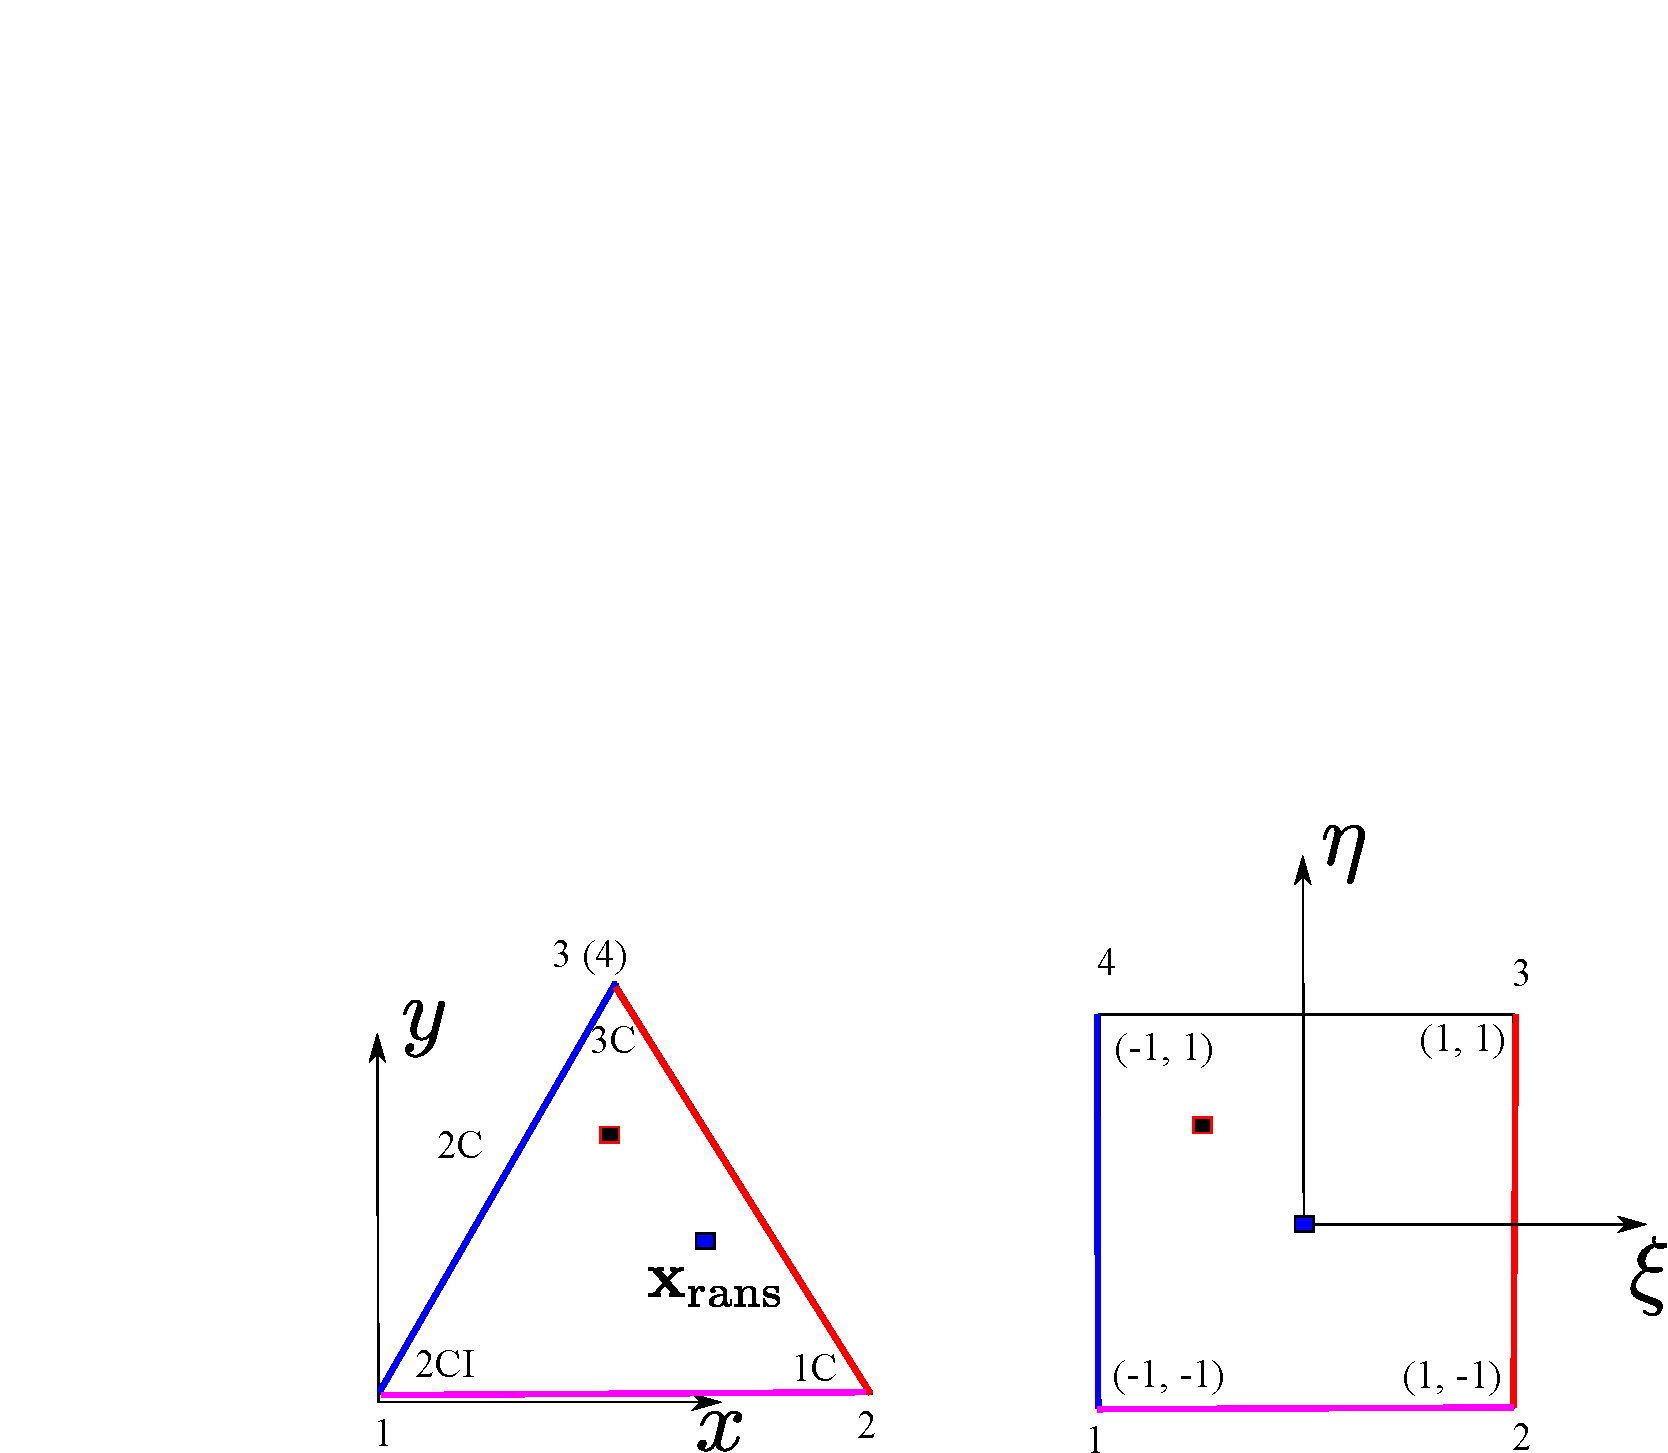
\includegraphics[width=0.8\textwidth]{quad2tri-mapping.pdf} \\
  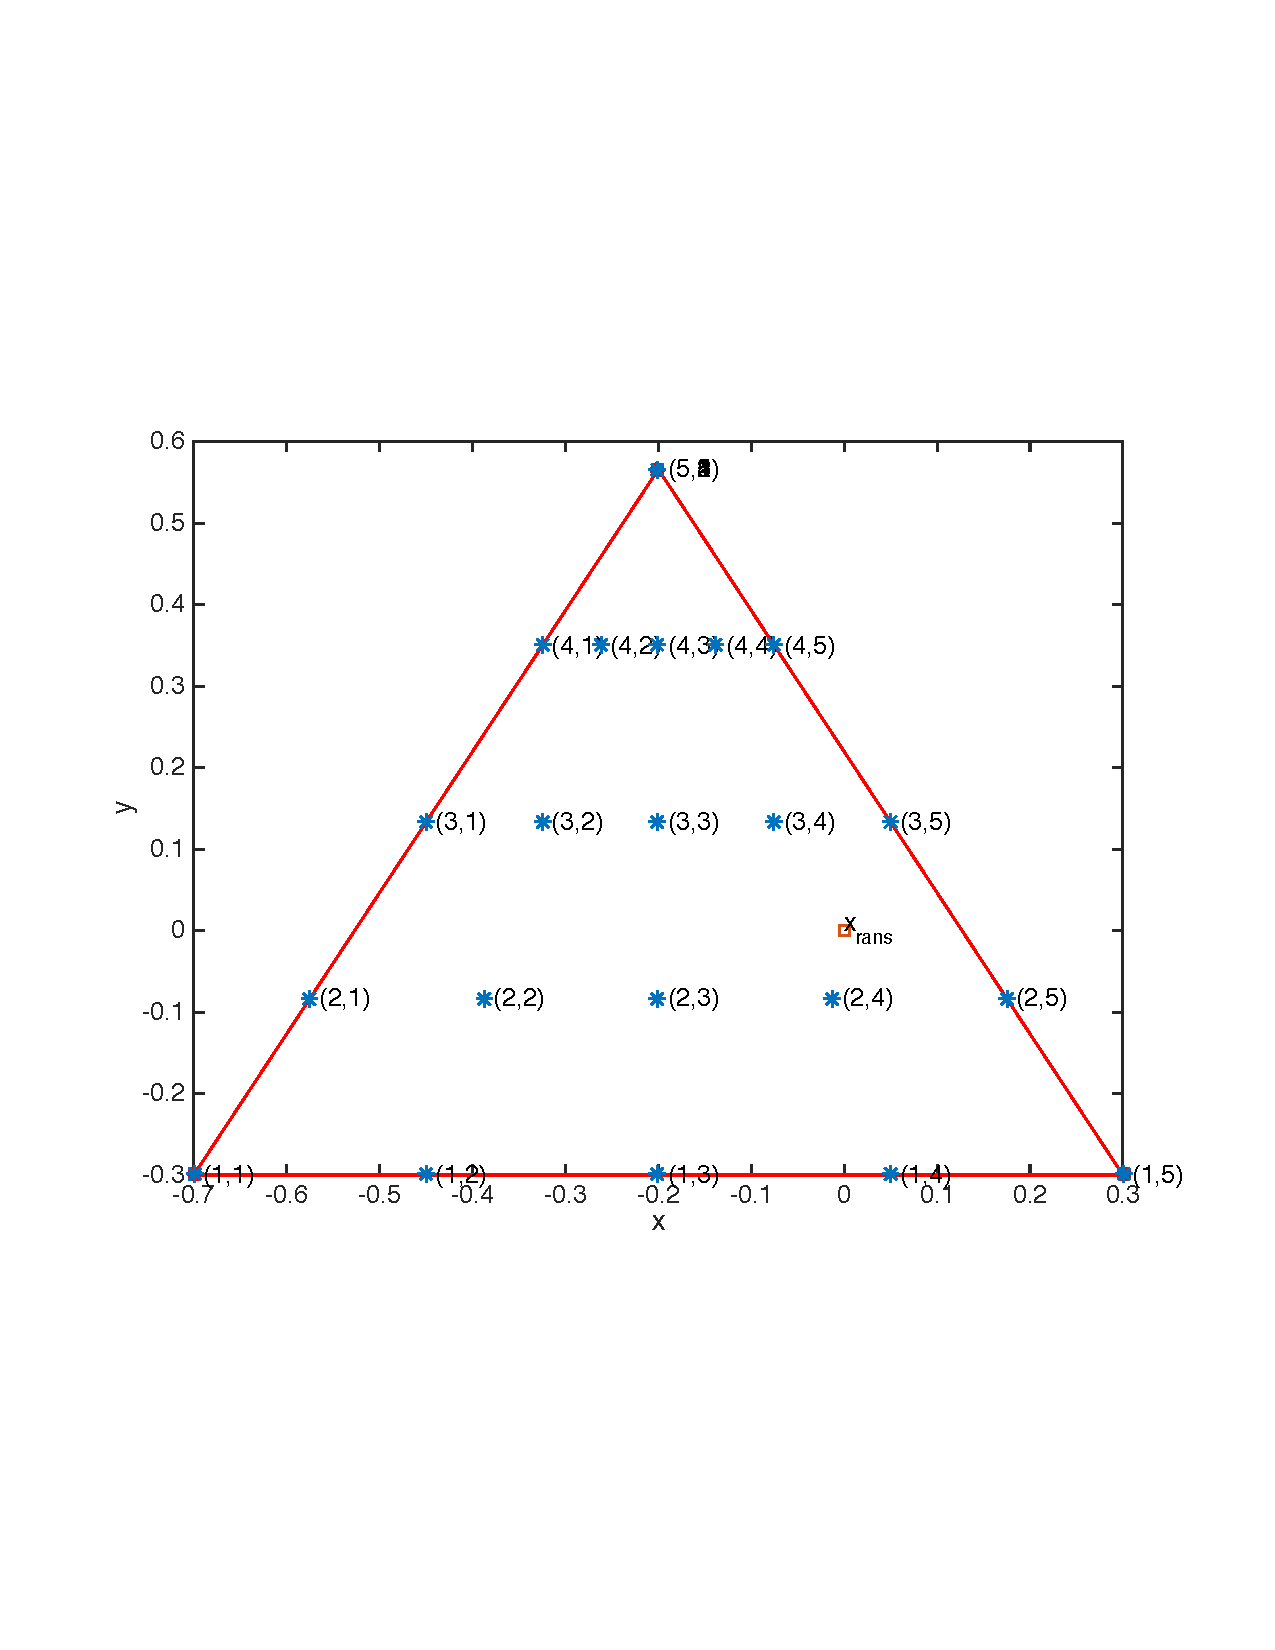
\includegraphics[width=0.49\textwidth]{physical.pdf}
  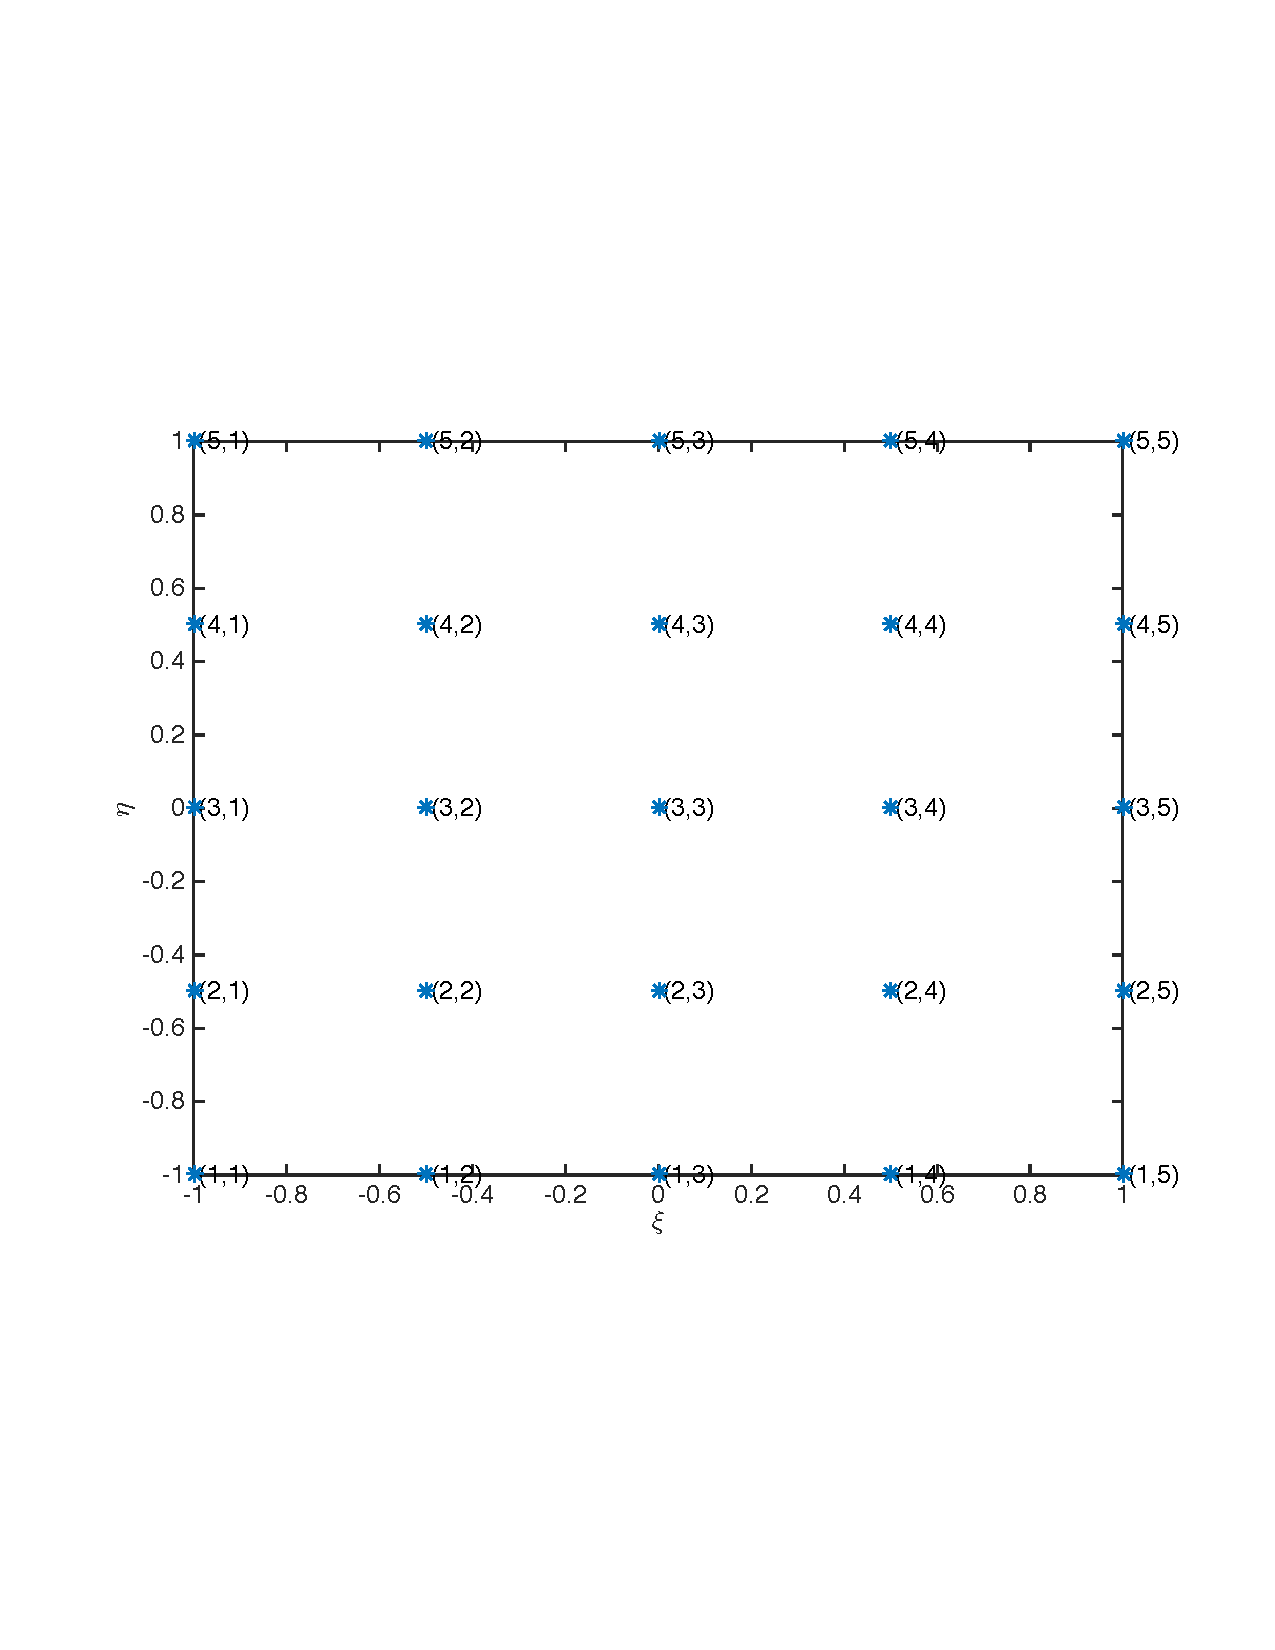
\includegraphics[width=0.49\textwidth]{mapped.pdf}
  \caption{Mapping between the Baycentric triangle to a unit square with original at the center. Top: Schematic showing the
    collapsing of node 1 and 2 (from the unit square) to node 1 in the physical domain. Color
    indicate correspondence. Bottom
    figures  are generated
    with \url{file://../../sandbox/quadMapping/tri2Square.m}.}
  \label{fig:phy-map}
\end{figure}



Other auxiliary functions include:
\assignment{JL:Auxiliary function about $\tau_{ij}$}{JL}{Implement and test the following functions in Items 1 to 2.}
\statusreport{}{Rui}{}


\begin{enumerate}
\item Check the physical realizability of entries in a field of Reynolds stresses, and plot on the
  Baycentric map (see Gorle et al., 2013). Will need to call function \verb+tau2PhysParams+ above.
\item Identify perturbation in Baycentric map, i.e., given an original $tau_{ij}$ and perturbed
  $tau^*_{ij}$, identify $\varphi$ and $\Delta$
\begin{python}
def perturbTaus(taus, tausPerturbed):
    """
    Input:
    taus, tausPerturbed
    Return:
    Array of psis and Deltas. 
    """
\end{python}
Ignore the difference of $k, v_1, v_2, v_3$ between the two Reynolds stresses, i.e., their amplitudes
and orientations. Only obtain their differences in ``shapes''.


\item Read Reynolds stress from OpenFOAM case file.
\begin{python}
def readTurbStressFromFile(tauName):
    """
    Input:
    path and file name of the Reynolds stress
    Return:
    Reynolds stress
    """
\end{python}

\item Write Reynolds stress to OpenFOAM file.
\begin{python}
def writeTurbStressToFile(taus, fileName):
    """
    Input:
    taus: list/array of Reynolds stress
    fileName: the destination file name
    Return:
    None
    """
\end{python}

\end{enumerate}

\subsection{Unit Tests}

\assignment{Rui/JL: Identify test cases}{Rui/JL}{Find a few physics-based test cases.}
\statusreport{Rui/JL: Assigned}{Rui/JL}{Assigned}

\commof{Document unit test results.}{XH}{Put some typical test results here as well.}

\section{Bayesian Inverse Modeling of Reynolds Stresses}


\subsection{Specification of Random Fields and Reduce Order Modeling}

\subsubsection{Theory}
The perturbation of the Reynolds stress, parameterized by $\varphi$ and $\Delta$ (i.e., relative polar
coordinate on the Baycentric map), are modeled as Gaussian processes, possibily with non-stationary
variance and length scales in the kernel function.

\begin{equation}
\Delta_\xi, \Delta_\eta \sim \mathcal{GP}(m(\mathbf{x}), K([\mathbf{x}-\mathbf{x}'])) 
\end{equation}
where
\begin{equation}
  \label{eq:kernel}
  K(\mathbf{x} - \mathbf{x}') = \sigma^2 \exp \left[  -\frac{(\mathbf{x}-\mathbf{x}')^2}{l^2}  \right]
\end{equation}
with $\sigma(\mathbf{x})$ and $l(\mathbf{x})$ being functions of $\mathbf{x}$, which is specified
beforehand via spline interpolation.  If Reynolds stresses at certain locations are available, they will be used to infer the
GP above.

For computational efficiency, Karhunen--Loeve expansion will be used to expand the Gaussian
process.\footnote{\url{http://www.mathworks.com/examples/matlab/3330-mercer-s-theorem-and-the-karhunen-loeve-expansion}.
  Also see: D. Xu, Numerical Methods for Stochastic Computations, Princeton University Press,
  2010.}.

\textbf{Theory from UQTk documentation}

\begin{equation}
F(t,\theta)  = \left < F(t,\theta) \right >_{\theta}                                                          
                + \sum_{k=1}^{\infty} \sqrt{\lambda_k} f_k(t) \xi_k 
\end{equation}

\begin{equation}
  \int C(s,t)f(t)dt  =\lambda f(s) \rightarrow \sum w_j C(s_i,t_j) f_k(t_j) = \lambda_k f_k(s_i)                  
\end{equation}

Further manipulation of the discretized Fredholm equation leads to the eigenvalue problem
\begin{equation}
  \label{eq:dis-ag}
A g=\lambda g  
\end{equation}
where $A=W K W$ and $g=Wf$, with $W$ being the diagonal matrix, $W_{ii}=\sqrt{w_i}$ and
$K_{ij}=Cov(t_i,t_j)$. Solutions consist of pairs of eigenvalues $\lambda_k$ and KL modes $f_k=W^{
  -1}g_k$.

\textbf{Description of functions in UQTK/KLDecompUni class}
\begin{enumerate}
\item \textit{void SetWeights(const Array1D$\langle$ double $\rangle$\& weights)}\\

Manipulate weight array (w\_(i) i from 0 to $n_t$ in the src code)

\item \textit{int decompose(const Array2D$\langle$ double $\rangle$\& corr, const int\& nKL)}\\

Perform KL decomposition into nKL modes and return actual number of modes that were obtained.

\item \textit{void KLproject(const Array2D$\langle$ double $\rangle$\& realiz, Array2D$\langle$ double $\rangle$\& xi)}\\

Project realizations $F(t,\theta_l)$ to the KL modes and store them in xi ($\xi_k$). Samples of random variables $\xi_k$ are obtained by projecting
  realizations of the random process $F$ on the eigenmodes $f_k$
   \[\left.\xi_k\right\vert_{\theta_l}=\left <F(t,\theta_l)-\left <
    F(t,\theta) \right >_{\theta}, f_k(t) \right >_t/\sqrt{\lambda_k} \]
  ... or numerically
  \[
  \left.\xi_k\right\vert_{\theta_l}=\sum_{i=1}^{N_p} w_i\left(F(t_i,\theta_l)-\left <
    F(t_i,\theta) \right >_{\theta} \right) f_k(t_i)/\sqrt{\lambda_k} \]

\item \textit{const Array2D$\langle$ double $\rangle$\& KLmodes() const}\\

Get associated KL modes

\item \textit{void meanRealiz(const Array2D$\langle$ double $\rangle$\& realiz, Array1D$\langle$ double $\rangle$\& mean\_realiz)}\\ 

Calculate (in meanRealiz) the mean realizations   

\item \textit{ void truncRealiz( const Array1D$\langle$ double $\rangle$\& meanrea, const Array2D$\langle$ double $\rangle$\& xi, const int\& nKL, Array2D$\langle$ double $\rangle$\& trunc\_realiz)}\\

Returns the truncated KL sum
 \[ 
    F(t_i,\theta_l) = \left < F(t_i,\theta) \right >_{\theta} 
                          + \sum_{k=1}^{nKL} \sqrt{\lambda_k} f_k(t_i) \left. \xi_k\right\vert_{\theta_l}
\] 


\end{enumerate} 




\subsubsection{Implementation Plan}
\assignment{JL/JX: Spline Interpolation}{JL/JX}{Use spline interpolation to obtain
  $\sigma(\mathbf{x})$ and $l(\mathbf{x})$.}
\statusreport{JL/JX: Assigned}{JL/JX}{Assigned.}

\begin{enumerate}
\item Specify values at a few chosen locations. Use spline to interpolate values in the entire
  field. Possible to borrow code from external sources or library. Start from 1D, and extend to 2D
  (or even 3D, eventually).
  \begin{python}
 def splineInterpolate(x, y, fieldX):
 """
 Input
 x: given coordinates
 y: given values
 (Maybe other parameters related to properties of the spline used for interpolation)
 fieldX: coordinate in the field
 Return: 
 fieldY: values corresponding to fieldX
 """
  \end{python}


\assignment{JX:Implementation and Testing of KL expansion}{JX}{Implementation and Testing of
  Karhunen--Loeve expansion. }
\statusreport{JX: Assigned}{JX}{Assigned.}

\item Implementation and testing of Karhunen--Loeve expansion. Test your implementation by drawing
  samples and verify their correlation against the kernel function you specified originally. Details
  in
  \footnote{\url{file:///Users/xiao/MobileOffice/software/UQTk_v2.1.1/examples_cpp/kl_sample/kl_example.pdf}
    The file is reproduced in reference folder.}.  Follow the example in Matlab, and start with 1D,
  extend to 2D (eventually to 3D later). For efficiency (both computational efficiency and
  implementation reliability), \emph{you should borrow code or directly use UQTK or MUQ}. MUQ used
  package ``Eigen''.  There is a test case on 2D irregular domain. Refer to \verb+kl_example.pdf+
  for details.

\begin{figure}[htbp]
  \centering
  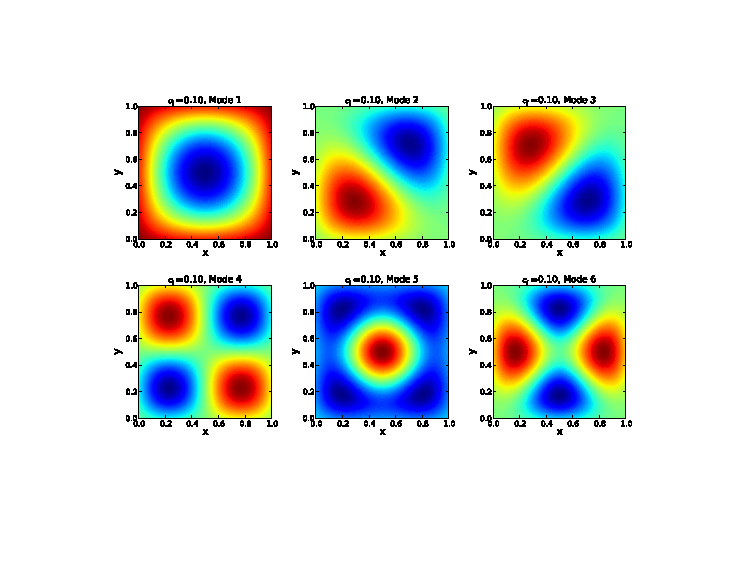
\includegraphics[width=0.8\textwidth]{KL-example-structured.pdf}
  \caption{Example of KL eigenmodes on a structured mesh. Picture taken from from UQTK.}
  \label{fig:box}
\end{figure}

\begin{figure}[htbp]
  \centering
  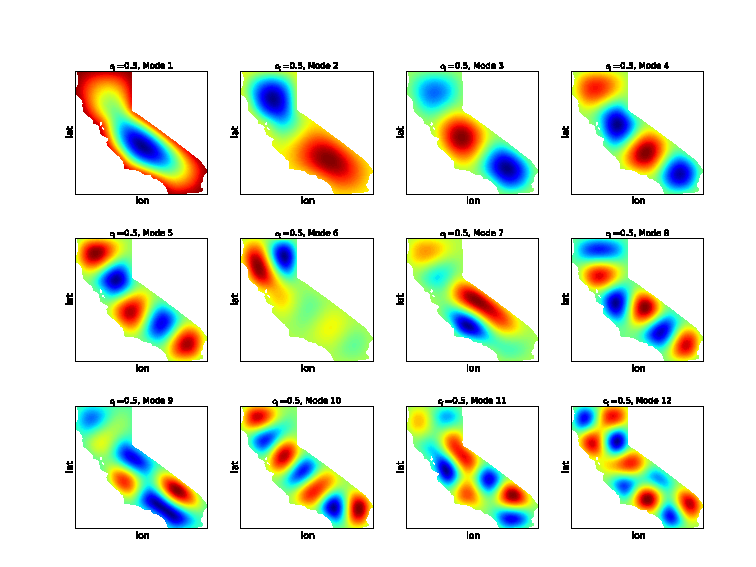
\includegraphics[width=0.8\textwidth]{KL-example-unstructured.pdf}
  \caption{Example of KL eigenmodes on a unstructured mesh (map of California). Picture taken from from UQTK.}
  \label{fig:cali}
\end{figure}

\end{enumerate}

\subsubsection{Unit Testing}


\subsection{Construction Prior for Reynolds Stresses Perturbation}

\subsubsection{Theory}
\subsubsection{Implementation Plan}
\subsubsection{Unit Testing}



\subsection{Inversion Methods}

\subsubsection{Theory}
We will explore two possible inverse modeling methods for now. New ideas will be added as they come up.
\begin{enumerate}
\item Ensemble Kalman Filtering (EnKF), which is an approximate method.
\item Markov Chain Monte Carlo (MCMC) with Delayed Rejection Adaptive Metropolis sampling (DRAM)
  algorithm\footnote{H. Haario, M. Laine, A. Mira and E. Saksman, 2006. DRAM: Efficient adaptive
    MCMC, Statistics and Computing 16, pp. 339-354. (doi:10.1007/s11222-006-9438-0).  Also see:
    \url{http://helios.fmi.fi/~lainema/mcmc/}}, which is more accurate but very expensive.
\end{enumerate}

\subsubsection{Implementation Plan}



\subsubsection{Unit Testing}
\commof{XH: Unit test results for inverse modeling}{XH}{Put the unit test results here.}



% \subsubsection{Theory}
% \subsubsection{Implementation Plan}
% \subsubsection{Unit Testing}


\section{Overall Algorithm}

The overall algorithm is as follows:

\begin{enumerate}
\item  Initialize mesh and specify initial and boundary conditions in OpenFOAM case.
\item \emph{Solve RANS}  Solve the ``nominal case'' to obtain baseline Reynolds stress $\tau^0_{ij}$ and velocity
  $\mathbf{u}^0$.

\item \emph{(Reynolds stress mapping)} Use a series of mapping to map $\tau^0_{ij}$ to natural
  coordinates ($\xi, \eta$).


  \emph{The following two steps are KL expansion procedure, i.e., reduced order modeling of random
    fields $\Delta_\xi$ and $\Delta_\eta$, or the Reynolds stress errors.} .

\item Specify kernel functions for the Gaussian processes of $\Delta_\xi$ and $\Delta_\eta$
  (corrections of Reynolds stress on the natural coordinate).
  
\item Perform KL expansion on the field $\Delta_\xi$ and $\Delta_\eta$ to obtain the coefficients
  $\omega_{\xi, i}$ and $\omega_{\eta, i}$ as well as modes $\lambda_i f_i(\mathbf{x})$, where $i =
  1 \cdots m$, and $m$ is the number of modes retained in the truncation. Assume $\omega_{\xi, i}$
  and $\omega_{\eta, i}$ have the same covariance and modes for now.

  The states are defined as $\mathbf{s} = [u, \boldsymbol{\omega}] $, where $u$ are the velocity of
  all cells; with
\[
\boldsymbol{\omega} \equiv [\omega_{\xi, 1}, \cdots, \omega_{\xi, m}, \omega_{\eta, 1},
\omega_{\eta, m}]
\]

\emph{The following steps are EnKF procedure.}

\item \emph{Sampling} Use sampled fields $\delta^1_\xi$ and $\delta^1_\eta$ to $\delta^m_\xi$ and
  $\delta^m_\eta$ to correct the baseline Reynolds stress $\tau^0_{ij}$ to obtain a certain number
  of Reynolds stress realizations $\tau^1_{ij}, \cdots, \tau^m_{ij}$. \label{it:sampling}

\item \emph{Forecasting} Use OpenFOAM to propagate all Reynolds stress realizations $\tau^1_{ij}, \cdots,
  \tau^m_{ij}$ to velocities. \label{it:solveRans}

\item \emph{Filtering/Analysis} Use EnKF procedure to compare propagated states with observations ($u$), and
  find analyzed states (corrections). New coefficients $\omega_\xi$ and $\omega_\eta$ will be
  obtained, along with new velocity fields. \label{it:analysis}

\item \emph{Reconstruction} Use the new coefficients $\boldsymbol{\omega}$ and the KL modes
  $\lambda_i f_i(\mathbf{x})$ saved before to generate new Reynolds stresses. \label{it:reconstruct}

\item Repeat Steps ~\ref{it:sampling} to \ref{it:reconstruct} until the EnKF procedure is converged.

\end{enumerate}

\section{Comprehensive Test Cases}

\assignment{Plot Reynolds stress on Baycentric triangle.}{JL/JX/Rui} {Choose a few cases with DNS
  data. Perform RANS on these cases, and plot DNS and RANS on the Baycentric triangle. }

Choose a few cases with DNS data. Perform RANS on these cases, and plot DNS and RANS on the
Baycentric triangle.  This would help us understand the Reynolds stress discrepancy, and postulate
prior distribution for $\varphi$ and $\Delta$. Cases with DNS or resolved LES data at least
include\footnote{J Jimenez, Moser, R. D., Tavoularis, S., \& Leuchter, O. (2009). A selection of
  test cases for the validation of large-eddy simulations of turbulent flows. AGARD ADVI SORY REPORT
  NO 345, 1-207. Available in Sente library. An online ftp provides the data. Some data are
  available in the archive of my JCP paper.}:
\begin{enumerate}
\item Channel flow with  $Re_\tau = 395$  and  $Re_\tau = 595$.
\item Periodic hill with $Re_b= 2800$ and $10595$.
\item Flow in a square duct.
\end{enumerate}


\subsection{Channel Flow with $Re_\tau = 595$ and $2003$}

\subsection{Flow over Periodic Hill at $Re_b= 2800$ and $10595$}

\appendix

\section{Contributions of Members by Tasks}
\assignment{Contribution table}{SR}{Make it a table.}
% e.g., as follows
% Task | JL | JX | Rui
% xxx  | x    | x    | x 
%  Task should have fixed width.

\begin{enumerate}
\item RANS solver development and testing:
\item Reynolds stress mapping, development and testing 
\item KL expansion development and testing:
\end{enumerate}



%\bibliographystyle{plain}
\bibliographystyle{ieeetr}
\bibliography{ref}
\end{document}